% !TEX root = ./notes_template.tex
%%%%%%%%%%%%%%%%%%%%%%%%%%%%%%%%%%%%%%%%%%%%%%%%%%
%%%%%%%%%%%%%%%%%%%%% preamble %%%%%%%%%%%%%%%%%%%
%%%%%%%%%%%%%%%%%%%%%%%%%%%%%%%%%%%%%%%%%%%%%%%%%%
\documentclass[11pt,twoside]{book}


\usepackage{luatex85}


\usepackage{ctex}
\renewcommand{\contentsname}{目录}
\usepackage{fontspec}
\usepackage{xeCJK}
\setCJKmainfont{LXGW WenKai Mono}
\linespread{1.5}


\usepackage{xeCJKfntef}
\xeCJKsetup{underdot/symbol={\normalfont^^b7}}
\newcommand{\dotemph}[1]{\CJKunderdot{#1}}





%\renewcommand{\baselinestretch}{1.05}
\usepackage{amsmath,amsthm,amssymb,mathrsfs,amsfonts,dsfont}
\usepackage{epsfig,graphicx}
\usepackage{tabularx}
\usepackage{blkarray}
\usepackage{slashed}
\usepackage{color}
\usepackage{listings}
\usepackage{caption}
% \usepackage{fullpage}
\usepackage{lipsum} % provides dummy text for testing
\usepackage[toc,title,titletoc,header]{appendix}
\usepackage{minitoc}
\usepackage{color}
\usepackage{multicol} % two-col ToC
\usepackage{bm}
\usepackage{imakeidx} % before hyperref
\usepackage{hyperref}
% link colors settings
\hypersetup{
    colorlinks=true,
    citecolor=magenta,
    linkcolor=magenta,
    filecolor=green,      
    urlcolor=cyan,
    % hypertexnames=false,
}
\usepackage[capitalise]{cleveref}
\usepackage{subcaption}
\usepackage{enumitem}
\usepackage{mathtools}
\usepackage{physics}
\usepackage[linesnumbered,ruled,vlined,algosection]{algorithm2e}
\SetCommentSty{textsf}
\usepackage{epigraph}
\epigraphwidth=1.0\linewidth
\epigraphrule=0pt

% adjust margin
\usepackage[margin=2.3cm]{geometry}
\headheight13.6pt

%%%%%%%%%%%%%%%% thmtools %%%%%%%%%%%%%%%%%%%%%
\usepackage{thmtools}
\declaretheorem[numberwithin=chapter]{theorem}
\declaretheorem[numberwithin=chapter]{axiom}
\declaretheorem[numberwithin=chapter]{lemma}
\declaretheorem[numberwithin=chapter]{proposition}
\declaretheorem[numberwithin=chapter]{claim}
\declaretheorem[numberwithin=chapter]{conjecture}
\declaretheorem[sibling=theorem]{corollary}
\declaretheorem[numberwithin=chapter, style=definition]{definition}
\declaretheorem[numberwithin=chapter, style=definition]{problem}
\declaretheorem[numberwithin=chapter, style=definition]{example}
\declaretheorem[numberwithin=chapter, style=definition]{exercise}
\declaretheorem[numberwithin=chapter, style=definition]{observation}
\declaretheorem[numberwithin=chapter, style=definition]{fact}
\declaretheorem[numberwithin=chapter, style=definition]{construction}
\declaretheorem[numberwithin=chapter, style=definition]{remark}
\declaretheorem[numberwithin=chapter, style=remark]{question}
%%%%%%%%%%%%%%%% thmtools %%%%%%%%%%%%%%%%%%%%%
\usepackage{changepage}
\newenvironment{solution}
    {\renewcommand\qedsymbol{$\square$}\color{blue}\begin{adjustwidth}{0em}{2em}\begin{proof}[\textit Solution.~]}
    {\end{proof}\end{adjustwidth}}

%%%%%%%%%%%%%%%% index %%%%%%%%%%%%%%%%%%%%%
\begin{filecontents}{index.ist}
% https://tex.stackexchange.com/questions/65247/index-with-an-initial-letter-of-the-group
headings_flag 1
heading_prefix "{\\centering\\large \\textbf{"
heading_suffix "}}\\nopagebreak\n"
delim_0 "\\nobreak\\dotfill"
\end{filecontents}
\newcommand{\myindex}[1]{\index{#1} \emph{#1}}
\makeindex[columns=3, intoc, title=Alphabetical Index, options= -s index.ist]
%%%%%%%%%%%%%%%% index %%%%%%%%%%%%%%%%%%%%%

%%%%%%%%%%%%%%%% ToC %%%%%%%%%%%%%%%%%%%%%
% Link Chapter title to ToC: https://tex.stackexchange.com/questions/32495/linking-the-section-text-to-the-toc
\usepackage[explicit]{titlesec}
% \titleformat{\chapter}[display]
%   {\normalfont\huge\bfseries}{\chaptertitlename\ {\thechapter}}{20pt}{\hyperlink{chap-\thechapter}{\Huge#1}
% \addtocontents{toc}{\protect\hypertarget{chap-\thechapter}{}}}
% \titleformat{name=\chapter,numberless}
%   {\normalfont\huge\bfseries}{}{-20pt}{\Huge#1}

  \titleformat{\chapter}[display]
  {\normalfont\huge\bfseries}{第\,\thechapter\,章}{20pt}{\hyperlink{chap-\thechapter}{\Huge#1}
\addtocontents{toc}{\protect\hypertarget{chap-\thechapter}{}}}



\titleformat{\subsubsection}[runin]
  {\normalfont\large\bfseries}{}{}{#1}[]




%%%%%%%%%%%%%%%%%%% fancyhdr %%%%%%%%%%%%%%%%%
\usepackage{fancyhdr}
\pagestyle{fancy} % enable fancy page style
\renewcommand{\headrulewidth}{0.0pt} % comment if you want the rule
\fancyhf{} % clear header and footer
\fancyhead[lo,le]{\leftmark}
\fancyhead[re,ro]{\rightmark}
\fancyfoot[CE,CO]{\hyperref[toc-contents]{\thepage}}

% https://tex.stackexchange.com/questions/550520/making-each-page-number-link-back-to-beginning-of-chapter-or-section
\makeatletter
\def\chaptermark#1{\markboth{\protect\hyper@linkstart{link}{\@currentHref}{Chapter \thechapter ~ #1}\protect\hyper@linkend}{}}
\def\sectionmark#1{\markright{\protect\hyper@linkstart{link}{\@currentHref}{\thesection ~ #1}\protect\hyper@linkend}}
\makeatother
%%%%%%%%%%%%%%%%%%% fancyhdr %%%%%%%%%%%%%%%%%


%%%%%%%%%%%%%%%%%%% biblatex %%%%%%%%%%%%%%%%%
\usepackage[doi=false,url=false,isbn=false,style=alphabetic,backend=biber,backref=true, minalphanames=3]{biblatex}

\DefineBibliographyStrings{english}{
  backrefpage={Cited on page},
  backrefpages={Cited on pages}
}

\addbibresource{bib.bib}

\DefineBibliographyStrings{english}{bibliography={参考文献}}

\newbibmacro{string+doiurlisbn}[1]{%
  \iffieldundef{doi}{%
    \iffieldundef{url}{%
      \iffieldundef{isbn}{%
        \iffieldundef{issn}{%
          #1%
        }{%
          \href{http://books.google.com/books?vid=ISSN\thefield{issn}}{#1}%
        }%
      }{%
        \href{http://books.google.com/books?vid=ISBN\thefield{isbn}}{#1}%
      }%
    }{%
      \href{\thefield{url}}{#1}%
    }%
  }{%
    \href{http://dx.doi.org/\thefield{doi}}{#1}%
  }%
}



% https://tex.stackexchange.com/questions/94089/remove-quotes-from-inbook-reference-title-with-biblatex
\DeclareFieldFormat[article,incollection,inproceedings,book,misc]{title}{\usebibmacro{string+doiurlisbn}{\mkbibemph{#1}}}
% https://tex.stackexchange.com/questions/454672/biblatex-journal-name-non-italic
\DeclareFieldFormat{journaltitle}{#1\isdot}
\DeclareFieldFormat{booktitle}{#1\isdot}
% https://tex.stackexchange.com/questions/10682/suppress-in-biblatex
\renewbibmacro{in:}{}
% add video field: https://tex.stackexchange.com/questions/111846/biblatex-2-custom-fields-only-one-is-working
\DeclareSourcemap{
    \maps[datatype=bibtex]{
      \map{
        \step[fieldsource=video]
        \step[fieldset=usera,origfieldval]
    }
  }
}
\DeclareFieldFormat{usera}{\href{#1}{\textsc{Online video}}}
\AtEveryBibitem{
    \csappto{blx@bbx@\thefield{entrytype}}{% put at end of entry
        \iffieldundef{usera}{}{\space \printfield{usera}}
    }
}
%%%%%%%%%%%%%%%%%%% biblatex %%%%%%%%%%%%%%%%%

%%%%%%%%%%%%%%%%%%%%% glossaries %%%%%%%%%%%%%%%%%
% !TEX root = ./notes_template.tex
% \usepackage[style=super]{glossaries}
% https://www.overleaf.com/learn/latex/Glossaries
\usepackage[style=super,toc,acronym]{glossaries}
\setlength{\glsdescwidth}{1\linewidth}
\makeglossaries

\renewcommand\glossaryname{List of Abbreviations and Symbols}

\newglossaryentry{Q2}{name={$Q_2(f)$},
%sort=Q2,
description={Two-side (bounded) error quantum query complexity}}

\newglossaryentry{real_number}{name={$\mathbb{R}$},description={Real number}}

% \newglossaryentry{gcd}{name={gcd},description={greatest common divisor}}

\newacronym{gcd}{GCD}{Greatest Common Divisor}


\newglossaryentry{svm}{name={SVM},description={Support Vector Machine}}

\newglossaryentry{gd}{name={GD},description={Gradient Descent}}

\newglossaryentry{qft}{name={QFT},description={Quantum Field Theory}}

\newglossaryentry{qm}{name={QM},description={Quantum Mechanics}}

\newglossaryentry{v}{name={$\vec{v}$},description={a vector}}

% physics
\newglossaryentry{hamiltonian}{name={$\hat{H}$},description={Hamiltonian}}

\newglossaryentry{lagrangian}{name={$L$},description={Lagrangian}}
%%%%%%%%%%%%%%%%%%%%% glossaries %%%%%%%%%%%%%%%%%

%%%%%%%%%%%%%%%%%%%%% glossaries-extra %%%%%%%%%%%%%%%%%
% \usepackage[record,abbreviations,symbols,stylemods={list,tree,mcols}]{glossaries-extra}
%%%%%%%%%%%%%%%%%%%%% glossaries-extra %%%%%%%%%%%%%%%%%


% !TEX root = ./notes_template.tex

%%%%%%%%%%%%%%%%%%%%%%%%%%%%%%%%%%%%
%%%%%%%%%%%%%%%%%%%%%%%%%%%%%%%%%%%%
% math
\let\iff\relax
\newcommand{\iff}{\text{ iff }}
\newcommand{\OPT}{\textup{OPT}}

% physics
\newcommand{\acreation}{a^\dagger}



%%%%%%%%%%%%%%%%%%%%%%%%%%%%%%%%%%%%%%%%%%%%%%%%%%
%%%%%%%%%%%%%%%% begin of document %%%%%%%%%%%%%%%
%%%%%%%%%%%%%%%%%%%%%%%%%%%%%%%%%%%%%%%%%%%%%%%%%%

\begin{document}

\title{\bf \huge 证明、论证与零知识}
\author{Kurt Pan}
\date{\today}
\maketitle
\setcounter{tocdepth}{2}
\setcounter{minitocdepth}{1} 

% \begin{multicols}{2}
    \dominitoc% Initialization
    \adjustmtc[2]% chp number shift for mini-toc
    \tableofcontents
    \label{toc-contents}
% \end{multicols}

% 	\listoffigures
% 	% \listoftables
% \begin{multicols}{2}
% 	\listoftheorems[ignoreall,show={theorem}]
% \end{multicols}

% 	\renewcommand{\listtheoremname}{List of Definitions}
% \begin{multicols}{2}
% 	\listoftheorems[ignoreall,show={definition}]
% \end{multicols}

	% \printglossaries
	% \printglossary[type=\acronymtype]
	% \printglossary
	% \printglossary[title=List of terms, toctitle=List of terms]

	% bib2gls
	% \printunsrtglossaries % print all types
	% \printunsrtglossary[type={abbreviations},title=List of Abbreviations,style=listgroup]
	% \printunsrtglossary[type={abbreviations},title=List of Abbreviations,style=listhypergroup] % doesn't work
	% \printunsrtglossary[type={symbols},title=List of Symbols,style=listgroup]
	% \printunsrtglossary % main entry

%%%%%%%%%%%%%%%Content%%%%%%%%%%%%%%%
% \mainmatter % separat the number of toc and mainmatter
% 原始模版内容
% % !TEX root = ../notes_template.tex
\chapter*{Preface}
\addcontentsline{toc}{chapter}{Preface}
\minitoc

% \lipsum % dummy text - remove from real document

\section{Features of this template}
% \epigraph{\emph{... nature isn't classical, dammit, and if you want to make a simulation of nature, you'd better make it quantum mechanical, and by golly it's a wonderful problem, because it doesn't look so easy.}}{Richard Feynman (1981) Simulating physics with computers}
\epigraph{\emph{TeX, stylized within the system as \LaTeX, is a typesetting system which was designed and written by Donald Knuth and first released in 1978. TeX is a popular means of typesetting complex mathematical formulae; it has been noted as one of the most sophisticated digital typographical systems.}}{- \href{https://en.wikipedia.org/wiki/TeX}{Wikipedia}}

\subsection{crossref}
different styles of clickable definitions and theorems
\begin{itemize}
	\item nameref:
		\nameref{def:gaussian_distribution}

	\item autoref:
		\autoref{def:gaussian_distribution},
		\autoref{alg:miller_rabin}

	\item cref:
		\cref{def:gaussian_distribution},

	\item hyperref:
		\hyperref[def:gaussian_distribution]{Gaussian},
\end{itemize}

\subsection{ToC (Table of Content)}
\begin{itemize}
	\item mini toc of sections at the beginning of each chapter
	\item list of theorems, definitions, figures
	\item the chapter titles are bi-directional linked
\end{itemize}

\subsection{header and footer}
fancyhdr
\begin{itemize}
	\item right header: section name and link to the beginning of the section
	\item left header: chapter title and link to the beginning of the chapter
	\item footer: page number linked to ToC of the whole document
\end{itemize}

\subsection{bib}
\begin{itemize}
	\item titles of reference is linked to the publisher webpage e.g., \cite{kitaev2002classical}
	\item backref (go to the page where the reference is cited) e.g., \cite{childsUniversalComputationQuantum2009}
	\item customized video entry in reference like in \cite{babaiGraphIsomorphismQuasipolynomial2016}
\end{itemize}

\subsection{preface, index, quote (epigraph) and appendix}
\myindex{index} page at the end of this document...

\subsection{symbol and glossary (abbreviation)}
examples: 
\gls{real_number},
% \gls{natural_number},
% \gls{complex_number},
\gls{svm},
\gls{v}

\subsubsection{usage}
\begin{itemize}
	\item glossary package 
	\begin{verbatim}
		pdflatex notes_template.tex
		makeglossaries notes_template
		pdflatex notes_template.tex	
	\end{verbatim}

	\item glossary-extra package and bib2gls
	\begin{verbatim}
		pdflatex notes_template.tex
		bib2gls notes_template
		pdflatex notes_template.tex	
	\end{verbatim}
\end{itemize}

\section{Related Tools}
\subsection{VSCode}
Extension: \href{https://marketplace.visualstudio.com/items?itemName=James-Yu.latex-workshop}{Latex Workshop by James Yu}

\subsubsection{settings}

\subsection{lualatex and latexmk}
.latexmkrc configuration file
\begin{verbatim*}
	$pdflatex = 'lualatex -synctex=1 -interaction=nonstopmode --shell-escape %O %S';
	@generated_exts = (@generated_exts, 'synctex.gz');
	$pdf_mode = 1;

	add_cus_dep('glo', 'gls', 0, 'makeglo2gls');
	sub makeglo2gls {
		system("makeindex -s '$_[0]'.ist -t '$_[0]'.glg -o '$_[0]'.gls '$_[0]'.glo");
	}
\end{verbatim*}
To explain ....
\begin{verbatim}
# Also delete the *.glstex files from package glossaries-extra. Problem is,
# that that package generates files of the form "basename-digit.glstex" if
# multiple glossaries are present. Latexmk looks for "basename.glstex" and so
# does not find those. For that purpose, use wildcard.
$clean_ext = "%R-*.glstex";

push @generated_exts, 'glstex', 'glg';

add_cus_dep('aux', 'glstex', 0, 'run_bib2gls');

# PERL subroutine. $_[0] is the argument (filename in this case).
# File from author from here: https://tex.stackexchange.com/a/401979/120853
sub run_bib2gls {
    if ( $silent ) {
    #    my $ret = system "bib2gls --silent --group '$_[0]'"; # Original version
        my $ret = system "bib2gls --silent --group $_[0]"; # Runs in PowerShell
    } else {
    #    my $ret = system "bib2gls --group '$_[0]'"; # Original version
        my $ret = system "bib2gls --group $_[0]"; # Runs in PowerShell
    };

    my ($base, $path) = fileparse( $_[0] );
    if ($path && -e "$base.glstex") {
        rename "$base.glstex", "$path$base.glstex";
    }

    # Analyze log file.
    local *LOG;
    $LOG = "$_[0].glg";
    if (!$ret && -e $LOG) {
        open LOG, "<$LOG";
    while (<LOG>) {
            if (/^Reading (.*\.bib)\s$/) {
        rdb_ensure_file( $rule, $1 );
        }
    }
    close LOG;
    }
    return $ret;
}
\end{verbatim}

\section{Copyright and License}

\begin{itemize}
    \item GitHub Repo: \url{https://github.com/Jue-Xu/Latex-Template-for-Scientific-Style-Book}
    \item Overleaf template: \url{https://www.overleaf.com/latex/templates/latex-template-for-scientific-style-book/ntprxjksmqxx}
\end{itemize}




% \part{Mathematics}
% % !TEX root = ../notes_template.tex
\chapter{Discrete Math}\label{chp:discrete_math}

\minitoc

gls example
\begin{itemize}
	% \item \glsxtrshort{gcd};
	\item \Gls{gcd}; \acrlong{gcd}; \acrshort{gcd}; \acrfull{gcd}
\end{itemize}

\section{Proof}
\begin{lemma}
\end{lemma}
\begin{claim}
\end{claim}
\begin{theorem}
\end{theorem}
\begin{example}
\end{example}
\begin{fact}
\end{fact}
\begin{remark}
\end{remark}
\begin{exercise}
	Prove A \iff B
\end{exercise}
\begin{solution}
By induction:
\end{solution}

\lipsum % dummy text - remove from real document

\section{Quantifier}
\lipsum % dummy text - remove from real document

\section{Graph}
\citetitle{babaiGraphIsomorphismQuasipolynomial2016}
\cite{babaiGraphIsomorphismQuasipolynomial2016}

\section{Number theory}
Figure example
\begin{figure}[!ht]
    \centering
    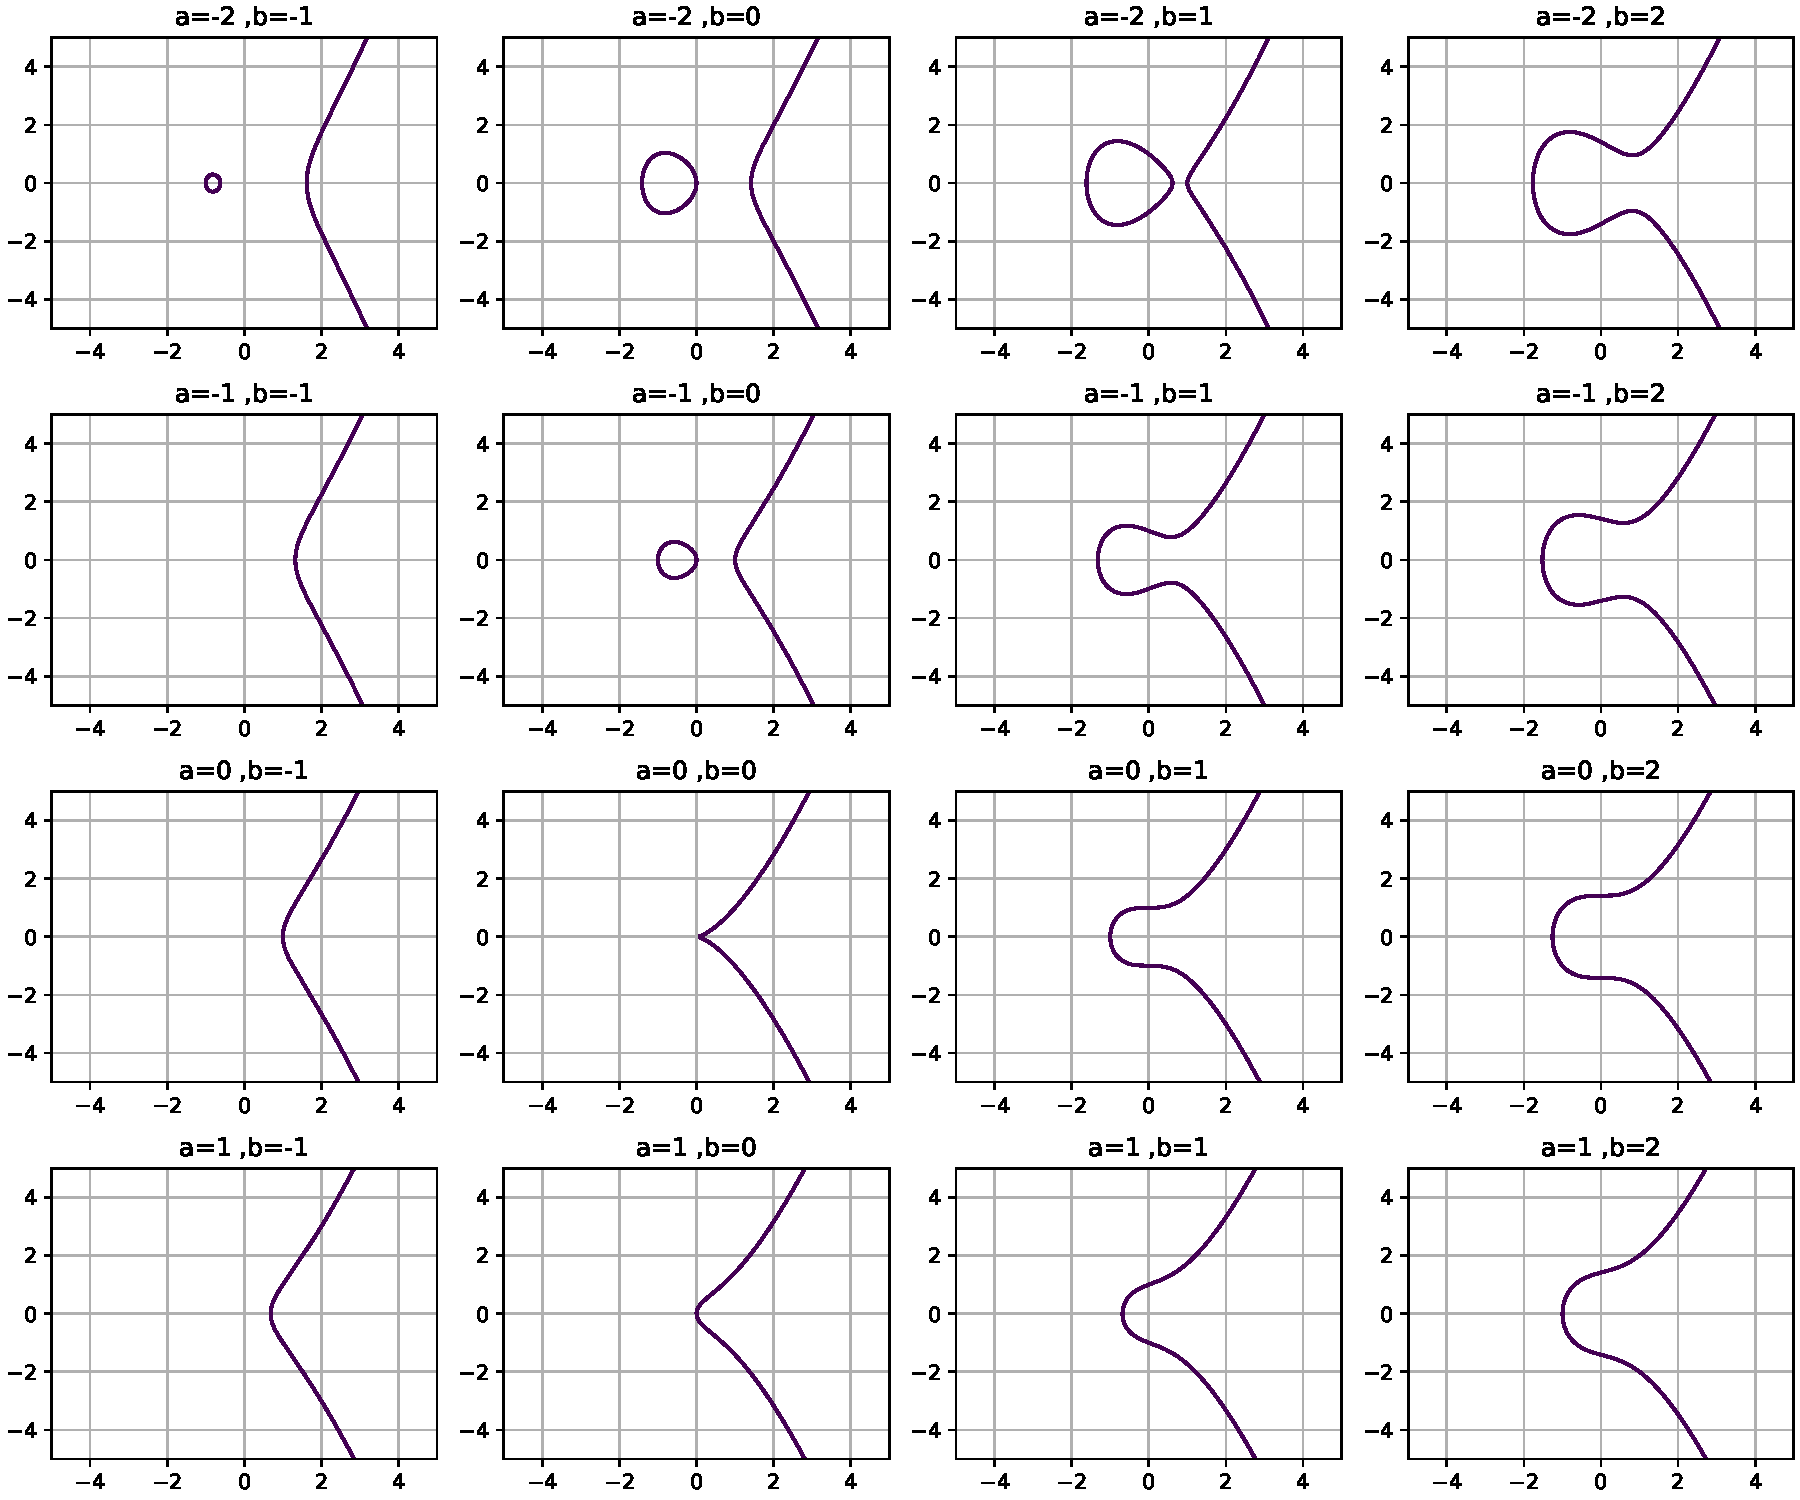
\includegraphics[width=1\linewidth]{./figure/elliptic_curves.pdf}
    \caption{Elliptic curves \cite{childsUniversalComputationQuantum2009} }
\end{figure}


\section{Algorithm}
% \begin{center}
% \begin{minipage}{.9\linewidth}
% algorithm2e
% https://www.overleaf.com/learn/latex/Algorithms#The_algorithm2e_package
\begin{algorithm}[H]
    \SetKwInOut{Input}{input}
    \SetKwInOut{Output}{output}
    \Input{Integer $N$ and parameter $1^t$}
    \Output{A decision as to whether $N$ is prime or composite}
    \BlankLine
    \For{ $i = 1,2, \ldots, t$} {
        $a\leftarrow \qty{1,\dots,N_1}$\;
        \If{$a^{N-1} \neq 1 \mod{N}$}
    {\Return "composite"}
    }
    \Return "prime"
    \caption{Primality testing - first attempt}
    \label{alg:miller_rabin}
\end{algorithm}
% \end{minipage}
% \end{center}

% \part{Computer Science}
% % \input{./chapter/complexity.tex}
% % !TEX root = ../notes_template.tex
\chapter{Machine Learning}\label{chp:machine_learning}
\minitoc

\section{Regression}
% \gls{algorithm};
\subsection{Gradient descent}\label{sec:gradient_descent}
\gls{gd};
% \glsxtrshort{gd}

\section{Support Vector Machine}
\gls{svm};
% % \input{./chapter/algorithms.tex}

% \part{Physics}
% % !TEX root = ../notes_template.tex
\chapter{Quantum Mechanics}\label{chp:quantum_mechanics}
\minitoc

\section{Hamiltonian}
\gls{hamiltonian};
% \glsxtrshort{qm};

\section{Path Integral}
\gls{lagrangian}

\section{Quantum Field Theory}
\gls{qft};
% % \input{./chapter/quantum_field_theory.tex}

% \begin{appendices}
%   % !TEX root = ../notes_template.tex
\chapter{Formulas}

\section{Gaussian distribution}\label{sec:gaussian_distribution}
\begin{definition}[Gaussian distribution]\label{def:gaussian_distribution}
    \myindex{Gaussian distribution}
\end{definition}

\begin{theorem}[Central limit theorem]\label{thm:central_limit_theorem}
\end{theorem}
%   \end{appendices}


\chapter{引言}\label{chp:01Introduction}


本书讨论了可验证计算(VC)。可验证计算是指一种名为交互式证明(IPs)和论证的密码学协议,证明者能够向验证者提供证明者正确地执行了所请求的计算的保证。交互式证明和论证在20世纪80年代被提出,代表了一个陈述为真的“证明”包括什么概念上的重大扩展。传统上的证明是一个静态对象,可以很容易地通过逐步检查来检验正确性,因为证明的每个单独步骤都应该易于验证。相比之下,交互式证明允许证明者和验证者之间的进行交互,以及允许无效证明以微小但非零的概率通过验证。交互式证明和论证之间的区别在于,论证(而非交互式证明)允许存在对错误陈述的“证明”,只要找到这些“证明”需要巨大的计算能力就可以。\footnote{比如说,一个不是IP的论证系统,可能会使用密码系统,使得作弊的证明者有可能找到一个可通过验证的对假陈述的“证明”,当且仅当证明者可以攻破密码系统。}

20世纪80年代中期和90年代初的著名理论结果表明,至少原则上讲,可验证计算协议可以达到惊人的成就:包括让手机可以去监控强大但不受信任(甚至恶意)的超级计算机的执行,让计算能力较弱的外设(例如,安全卡读卡器)将安全核心工作外包给强大的远程服务器,以及让数学家仅通过查看所谓证明中的几个符号就能对定理的正确性具有很高的信心。\footnote{只要证明以一种特定的、略微有些冗余的形式书写。具体见第\ref{chp:09PCP}章中对概率可检验证明(PCPs)的讨论。}


当VC协议具有一种称为\dotemph{零知识} 的性质时,它会在密码学环境中非常有用。零知识的意思是证明或论证除了其本身的有效性之外,不会泄露任何信息。

为了具体说明为什么零知识协议有用,考虑以下来自身份认证的典型例子。假如Alice选择了一个随机口令$x$,公开了一个哈希值$z=h(x)$。其中$h$是一个单向函数,给定一个对随机选择$x$ 的 $z=h(x)$, 需要大量计算能力才能找到 $z$ 在 $h$ 下的原像, 即一个满足 $h\left(x^{\prime}\right)=z$ 的 $x^{\prime}$。 
假如Alice 在之后想要说服 Bob 她是发布 $z$ 的同一个人。她可以通过向 Bob 证明她知道一个满足 $h\left(x^{\prime}\right)=z$ 的 $x^{\prime}$ 来实现这一点。这将使 Bob 相信 Alice 是发布 $z$ 的同一个人, 因为这意味着 Alice 要么一开始就知道 $x$, 要么她反转了 $h$ (这被认为是超出了 Alice 的计算能力)。

Alice 如何让 Bob 相信她知道 $h$ 下 $z$ 的原像? 一个简单的证明是 Alice 将 $x$ 发送给 Bob,Bob 可以轻松检验 $h(x)=z$。 但这样所揭示的信息比 Alice 知道 $z$ 的原像要多得多。 具体来说它揭示了原像本身。 Bob 可以使用该知识永远冒充 Alice,因为现在他也知道 $z$ 的原像了。

为了防止 Bob 获悉可能泄露口令 $x$ 的信息,给出不能揭示任何超出其自身有效性的内容的证明是很重要的。 这正是零知识性质所保证的。

本书的一个特定目标是描述构造所谓的零知识简洁非交互式知识论证(简称 zk-SNARKs)的各种方法。 “简洁”意味着证明很短。 “非交互”意味着证明是静态的,由来自证明者的单个消息组成。 (第二个)“知识”大致意味着协议不仅确定一个陈述为真,而且证明者\dotemph{知晓}一个“证据”来证明该陈述为真。 \footnote{例如,上述身份验证场景中确实需要对“存在一个口令 $x$ 使得 $h(x)=z$”这一陈述进行零知识\dotemph{知识}证明。 这是因为应用要求 Bob 不仅要确信在 $h$ 下\dotemph{存在} $z$ 的原像 $x$(如果 $h$ 是满射函数,这将始终为真),而且还要确信Alice 知道 $x$。}满足所有这些性质的论证系统在整个密码学中有无数应用。

对密码学相关的高度特定化的陈述(如证明离散对数的知识\cite{Sch89})的实用零知识协议已经有了数十年了。然而,通用零知识协议直到最近才变得足够高效,可以用于密码部署中。通用的意思是,协议设计技术适用于任意计算。这一令人兴奋的进展包括了漂亮的新协议的提出,并引发了各界对零知识证明和论证的浓厚兴趣。本书旨在以统一的方式让人们能够轻松理解这些协议设计的主要思想和方法。

\subsubsection{背景和上下文} 在20世纪80年代中期和90年代,理论计算机科学家理论计算机科学家发现IP 和论证系统可以比传统的静态和信息论安全 \footnote{信息论安全}的 $\mathbf{NP}$ 证明(至少在渐近意义上)更高效 。
刻画这些协议能力的基础定理(例如 $\mathbf{IP=PSPACE}$ \cite{LFKN92,Sha92}、$\mathbf{MIP=NEXP}$ \cite{BFL91} 和 PCP 定理 \cite{ALM+98,AS98})都是计算复杂性理论中最具影响力和最著名的定理。 \footnote{The results IP=PSPACE and MIP=NEXP are both covered in this survey (see Sections 4.5.5 and 8.5 respectively).}




\subsubsection{零知识协议设计方法及本书的理念}  
论证系统通常分两步开发。 
开发一个信息论安全协议(例如 IP、\dotemph{多证明者交互式证明} (MIP) 或\dotemph{概率可检查证明} (PCP)),以对单个或多个证明者假定以某种受限方式行事建模。(例如,在 MIP 中,会假定证明者不会相互发送有关他们从验证者那里收到的挑战的信息)。 
第二步,信息论安全的协议与密码学相结合,以“强制”(单个)证明者以受限方式行事,从而产生一个论证系统。 这第二步通常还会赋予所生成的论证系统重要的性质,例如零知识、简洁性和非交互性。 如果生成的论证系统满足所有这些性质,那么它实际上是一个 zk-SNARK。

\subsubsection{本书中信息论安全模型的顺序} 
我们首先介绍 IP,然后是 MIP,然后是 PCP 和 IOP,再然后是线性 PCP。 该顺序大致遵循研究文献中模型出现的时间顺序。 有点讽刺的是,这些模型是以类似于\dotemph{倒}时间序的方式应用于实际的 SNARK 设计中的。 比如说第一个实用的 SNARK 就是基于线性 PCP 的。 事实上这并非巧合:引入线性 PCP 的主要动机就是为了得到更简单和更实用的简洁论证,特别是考虑到从 PCP 导出的论证的\dotemph{实际不可用性}。


\subsubsection{逐章大纲}
\subsubsection{阅读本书的建议} 本书当然可以愉快地从头读到尾,但非线性路径可能会是一个更快地提供全面了解 SNARK 设计技术的途径。 为此提出的建议如下。

第 \ref{chp:02Randomness} 章和第 \ref{chp:03Definition} 章介绍了贯穿所有后续章节的基础技术概念(有限域、IP、论证、低次扩展、Schwartz-Zippel 引理等),不熟悉这些概念的读者不应跳过。

读者接下来可能希望阅读\dotemph{最后}一章,第\ref{chp:19SNARK}章,这章提供了所有 SNARK 设计方法及其相互关系的鸟瞰图。 第\ref{chp:19SNARK}章使用了一些读者此时可能不熟悉的术语,但仍然应该是可以理解的,并且其所提供的上下文对阅读更多技术章节会有所帮助。

在那之后,本书有很多可能的阅读路径。 对最先部署在商业环境中的 SNARK 特别感兴趣的读者可参阅第 \ref{chp:17LPCP} 章关于线性 PCP 的内容。 除了使用了第 \ref{15.1} 节介绍的基于配对的密码学(以及最后对零知识的处理,这是第 \ref{chp:11ZKP} 章正式介绍的一个概念)之外,本章基本上是独立的,

或者,读者可以转向理解 SNARK 设计的另一种方法,即去结合\dotemph{多项式} \emph{IOP}(IP、MIP 和 PCP 是其特例)和\dotemph{多项式承诺方案}。

为了快速理解多项式 IOP,建议仔细阅读第 \ref{4.1} 节关于和校验协议的内容,然后是第 \ref{4.6} 节关于用于电路求值的 GKR 交互式证明协议,或第 \ref{8.2} 节给出的电路可满足性的 2-证明者 MIP。 
接下来,读者可以翻到第 \ref{chp:07argfromip} 章,其中解释了如何将此类协议与多项式承诺结合起来以获得简洁论证。

要理解多项式承诺方案,读者可以阅读第 \ref{10.4} 和 \ref{10.5} 节以了解基于 IOP 的多项式承诺,或者转向第 \ref{chp:12sigma} 章和第 \ref{chp:14PCDL}-\ref{chp:16PC} 章(按此顺序)以了解基于离散对数问题和配对的多项式承诺。

本书网页\footnote{\url{https://people.cs.georgetown.edu/jthaler/ProofsArgsAndZK.html}}上发布的一系列三个视频提供了关于多项式 IOP 和多项式承诺的概述。 读者可能会发现在详细阅读第 \ref{chp:04IP}-\ref{chp:10IOP} 章之前观看这些视频会很有用。



\subsubsection{首次阅读可跳过的材料} Sections 4.2-4.5 are devoted to detailed example applications of the sum-check protocol and explaining how to efficiently implement the prover within it. While these sections contain interesting results and are useful for familiarizing oneself with the sum-check proto- col, subsequent chapters do not depend on them. Similarly, Chapter 5 on the Fiat-Shamir transformation and Chapter 6 on front-ends are optional on a first reading. Sections 9.3 and 9.4 provide PCPs that are mainly of historical interest and can be skipped.
Chapters 11 and 13 offer treatments of zero-knowledge that largely stand on their own. Similarly, Chapter 18 discusses SNARK composition and stands on its own.



\section{数学证明}
本书涵盖了\dotemph{数学证明}的不同概念及其在计算机科学和密码学中的应用。非正式地,我们所说的证明是指任何能使某人相信某项陈述为真的东西,而“证明系统”是指任何判定什么是令人信服的证明的程序。也就是说,证明系统由验证程序决定,该验证程序将任何陈述和声称该陈述为真的“证明”作为输入,判定该证明是否有效。

我们希望证明系统具有哪些性质呢?这有四个比较明显要有的。
\begin{itemize}
    \item 任何真陈述都应该有对其有效性的令人信服的证明。此性质通常称为\dotemph{完备性}。
    \item 任何假陈述都不应有令人信服的证明。此性质称为\dotemph{可靠性}。
    \item 理想情况下,验证程序将是“高效的”。 粗略地说,这意味着对简单的陈述应该有简短的(令人信服的)证明,且可以快速\dotemph{检验}。
    \item 理想情况下,证明生成也应该是高效的。 粗略地说,这意味着对简单的陈述应该有可以快速\dotemph{找到}的(令人信服的)短证明。
\end{itemize}


传统上,数学证明是可以逐行撰写并逐行检验其正确性的东西。 这种传统的证明概念正是复杂性类 $\mathbf{N P}$ \footnote{粗略地说,复杂性类 $\mathbf{N P}$ 包含所有这样的问题:任意输入上的正确答案为“是”或“否”,且对于所有“是”实例,存在一个有效可检验的(传统)证明,该证明的正确答案为“是”。 详细信息可参阅第 \ref{3.3} 节。} 所刻画的概念。但是在过去的30多年里,计算机科学家研究了更通用和更奇异的证明概念。这改变了计算机科学家对证明某事意味着什么的观念,并导致了复杂性理论和密码学的重大进步。


\section{我们将研究哪些非传统证明?}
本书中研究的所有证明概念本质上都是概率性的。
即验证程序将做出随机选择,且可靠性将以(非常)高的概率在这些随机选择上成立。 
也就是说,验证程序会以(非常)小的概率宣布假陈述为真。

\subsection{交互式证明 (IP)}
要理解什么是交互式证明,考虑以下应用场景可能会有帮助。 想象一家企业(验证者)使用某云计算提供商来存储和处理其数据。 
企业将其所有数据发送并存储到云(证明者),企业仅存储非常小的数据的“秘密”摘要(云不知道用户的秘密摘要)。 
随后,企业向云询问有关其数据的问题,通常以计算机程序$f$的形式提出,即企业希望云使用庞大的计算基础设施在其数据上运行该程序。 
云这样做了之后向用户发送程序的输出 $f(\text{数据})$。 企业可以使用交互式证明系统 (IP) 来获得该输出正确性的一个正式\dotemph{保证},而不是盲目地去相信云在数据上正确执行了该程序。

在 IP 中,企业询问云,发送一系列挑战并接收一系列响应。 在询问结束时,企业必须决定是接受有效答案还是拒绝无效答案。 有关此交互的图,请参见图 1.1。

IP 的完备性保证了如果云在数据上正确运行了程序并遵循所规定的协议,那么用户将被说服接受有效的回答。 IP 的可靠性保证了如果云返回错误的输出,那么\dotemph{无论云如何努力诱使用户}接受回答为有效,用户都将以很高概率拒绝回答为无效。 直观上,IP 的交互本质使得企业可以利用意外元素(即云无法预测企业的下一个挑战这一事实)来捕捉到云的谎言。

值得一提的是 IP 和传统静态证明之间的一个有趣区别。静态证明是\dotemph{可传递}的,如果 Peggy(证明者)向 Victor(验证者)提供一个陈述为真证明,Victor 可以继续去说服 Tammy(第三方)相同的陈述为真,只需复制证明即可。 反之,一个交互式证明是不可传递的。 Victor 可以通过向 Tammy 发送他与 Peggy 的交互脚本来尝试说服 Tammy 该陈述为真,但 Tammy 并不会被说服,除非 Tammy 相信 Victor 正确地代表了交互过程。 这是因为 IP 的可靠性仅在每次 Peggy 向 Victor 发送响应时,Peggy 不知道 Victor 接下来将响应什么挑战时才成立。 仅凭脚本并不能向Tammy保证这一点。

\subsection{论证系统}
论证系统就是IP,只是其中的可靠性性要求只需要防止在多项式时间内运行的作弊证明者。\footnote{这大致意味着如果输入的大小为 $n$,那么证明者的运行时间(对于足够大的 $n$ 值)应该以 $n$ 的某个常数幂为界,例如 $n^{10} $。}
论证系统会使用密码学。 
粗略地说,在论证系统中,作弊证明者无法欺骗验证者接受假陈述,除非它攻破了某个密码系统,且破解该密码系统被认为需要超多项式时间。

\subsection{多证明者交互式证明(MIP)/概率可检验证明(PCP)等}
MIP 类似于 IP,但有多个证明者,并且假设这些证明者不会相互共享他们从验证者那里收到的挑战的信息。 MIPs 的一个常见类比是在审讯之前将两名或更多犯罪嫌疑人放在不同的房间里,看他们是否能讲出一致的故事。 
执法人员可能不会对MIPs的研究为这种做法提供了理论依据感到太意外。
具体来说,MIPs的研究表明,将证明者锁在不同的房间里,然后分别审问他们,这可以说服审问者相信比在一起审问时更复杂的陈述。


在 PCP 中,证明与传统数学证明一样是静态的,但验证者只能从证明中读取少量(可能是随机选择的)字符。 \footnote{更准确地说,PCP验证者去读证明中尽可能多的内容是可以的。 然而,仅在验证者只需要阅读证明的一小部分即可高置信度地确定证明是否有效的情况下,才认为PCP是高效的。} 这类似于数学期刊的懒惰审稿人,他并不想费力地检查提交论文中的证明是否正确。 
PCP 定理 \cite{ALM+98,AS98}本质上指出,\dotemph{任何}传统的数学证明都可以写成特定格式,使这个懒惰的审阅者能够仅通过检查其中的几个词而对证明的有效性获得高度信心。

哲学上讲,MIP 和 PCP 都是非常有趣的研究对象,但它们并不能直接应用于大多数密码学场景中,因为它们对证明者(们)做出了不切实际或繁琐的假设。 
例如,任何 MIP 的可靠性仅在证明者不相互共享有关他们从验证者那里收到挑战的信息时才成立。 这在大多数密码学场景中并不直接有用,因为通常在这些场景中只有一个证明者,即使有多个证明者,也没有办法强制证明者不进行通信。 
类似地,虽然验证者只需读取 PCP 的几个字符,但一个PCP的直接实现却需要证明者将整个证明传输给验证者,这将是大多数现实场景中的主要开销所在(尽管例子中有一个懒惰的期刊审稿人)。 也就是说,一旦证明者将整个证明传输给验证者了,再让验证者避免阅读整个证明几乎没有什么现实世界的好处。

然而,通过将 MIP 和 PCP 与密码学相结合,我们将看到如何将它们变成论证系统,这些论证系统\dotemph{可以}直接应用于密码学场景。 例如,我们将在 \ref{9.2} 节中看到如何将 PCP 变成一个论证系统,在该系统中,证明者\dotemph{不必}将整个 PCP 发送给验证者。

本书的第 \ref{10.2} 节实际上提供了一个统一的抽象,称为\dotemph{多项式}\emph{IOP},在其中所有 IP、MIP 和 PCP 都是一个特例。 实际上,通过称为多项式承诺方案的密码学原语,任何多项式 IOP 都可以转换为具有短证明的论证系统。
\chapter{随机性的力量:指纹识别和 Freivalds 算法}\label{chp:02Randomness}

\section{Reed-Solomon指纹识别}\label{2.1}
\section{Freivalds算法}\label{2.2}
\section{看待指纹识别和Freivalds算法的另一种视角}\label{2.3}
\section{单变量Lagrange插值法}\label{2.4}
\chapter{定义和技术预备知识}\label{chp:03Definition}
\section{交互式证明}\label{3.1}
\section{论证系统}\label{3.2}
\section{定义的健壮性及交互式的威力} \label{3.3}
\section{Schwartz-Zippel引理}\label{3.4}
\section{低次和多线性扩展}\label{3.5}
\section{习题}\label{3.6}

\chapter{交互式证明系统}\label{chp:04IP}
\section{和校验协议}\label{4.1}
\section{和校验的首个应用:$^\# \mathrm{SAT} \in \mathbf{I P}$}\label{4.2}
\section{第二个应用:一个清点图中三角形数量的简单IP}\label{4.3}
\section{第三个应用:对矩阵乘法的非常高效的IP}\label{4.4}
\section{对矩阵乘法的非常高效的IP的应用}\label{4.5}
\section{GKR协议及其高效实现}\label{4.6}
\section{习题}\label{4.7}
\chapter{使用Fiat-Shamir得到公开可验证非交互式论证}\label{chp:05FS}

\section{随机预言模型} \label{5.1}
\section{Fiat-Shamir 转换} \label{5.2}
\section{转换的安全性} \label{5.3}
\section{习题} \label{5.4}

\chapter{前端:将计算机程序转化为电路}\label{chp:06FrontEnds}

\section{引言}\label{6.1}
\section{机器代码}\label{6.2}
\section{将程序转换为电路的第一个技术(概览)}\label{6.3}
\section{将小空间程序转换为浅电路}\label{6.4}
\section{将计算机程序转换为电路可满足性实例}\label{6.5}
\section{另外的转换和优化}\label{6.6}
\section{习题}\label{6.7}
\chapter{基于交互式证明的首个电路可满足性简洁论证}\label{chp:07argfromip}

\section{朴素方法:一个对电路可满足性的IP}\label{7.1}
\section{对电路可满足性的简洁论证}\label{7.2}
\section{第一个对电路可满足性的简洁论证}\label{7.3}
\section{知识可靠性}\label{7.4}
\chapter{MIP和简洁论证系统}\label{chp:08MIP}
\chapter{PCP和简洁论证系统}\label{chp:09PCP}

\section{PCP:定义及和MIP的关系}\label{9.1}
\section{将PCP编译为简洁论证系统}\label{9.2}
\section{基于MIP的首个多项式长度的PCP}\label{9.3}
\section{对算术电路可满足性的准线性长度PCP}\label{9.4}
\chapter{交互式预言证明}\label{chp:10IOP}
\chapter{零知识证明和论证系统}\label{chp:11ZKP}

\section{什么是零知识证明?}\label{11.1}
零知识证明或论证的定义刻画了这样一个概念,即验证者除了被证明的陈述的有效性之外,不应该从证明者那里学到任何东西。 \footnote{回顾一下,一个证明系统满足统计可靠性,而一个论证系统满足计算可靠性。 参见定义 \ref{def:3.1} 和 \ref{def:3.2}。} 
也就是说,验证者通过与诚实的证明者交互中学到的任何信息,都可以由验证者自己学到,而无需访问证明者。 
这需要通过模拟来形式化的,即要求有一种称为\dotemph{模拟器}的有效算法,该算法仅输入要证明的陈述,产生的脚本分布与和验证者与一个诚实证明者交互时产生的脚本分布无法区分(回顾 \ref{3.1} 节,交互式协议的脚本指协议执行期间证明者和验证者交换的所有消息的列表)。

\begin{definition}[零知识的非正式定义] \label{def:11.1}
    对于语言 $\mathcal{L}$,一个具有证明者 $\mathcal{P}$ 和验证者 $\mathcal{V}$ 的证明或论证系统被称为是零知识的,如果对于任意概率多项式时间验证者策略 $\hat{V}$,存在一个概率多项式时间算法 $S$(可以依赖于 $\hat{V}$),称为模拟器,使得对于所有 $x \in \mathcal{L}$ ,模拟器的输出分布$S(x)$ 与 $\operatorname{View}_{\hat{V}}(\mathcal{P}(x), \hat{V}( x))$“不可区分”。 $\operatorname{View}_{\hat{V}}(\mathcal{P}(x), \hat{V}(x))$ 表示由证明或论证系统中的证明者策略 $\mathcal{P}$ 和验证者策略 $\hat{V}$交互产生的脚本的分布。
\end{definition}

非正式地说,模拟器的存在意味着除了学习到 $x \in \mathcal{L}$ 之外,验证者 $\mathcal{V}$ 不会从证明者那里学到任何超出 $\mathcal{V}$ 可以自己高效地计算的东西。 
这是因为,以$x$ 在 $\mathcal{L}$ 中为条件,$\mathcal{V}$ 无法区分通过与诚实证明者交互生成的脚本与通过忽略证明者并运行模拟器所生成的脚本。 
因此,验证者可以从证明者那里学到的任何信息也可以从模拟器中学到(这是一个高效程序,因此验证者可以负担得起自己运行模拟器)。

定义\ref{def:11.1}中的术语“不可区分”有三种自然的意义:

\begin{itemize}
    \item One possibility is to require that $S(x)$ and $\operatorname{View}_{\hat{V}}(\mathcal{P}(x), \hat{V}(x))$ are literally the same distribution. In this case, the proof or argument system is said to be perfect-zero knowledge..$^{134}$
    \item Another possibility is to require that the distributions $S(x)$ and $\operatorname{View}_{\hat{V}}(\mathcal{P}(x), \hat{V}(x))$ have negligible statistical distance. In this case, the proof or argument system is said to be statistical zero-knowledge. Here, the statistical distance (also called total variation distance) between two distributions $D_1$ and $D_2$ is defined to be
    $$
    \frac{1}{2} \sum_y\left|\operatorname{Pr}\left[D_1(x)=y\right]-\operatorname{Pr}\left[D_2(x)=y\right]\right|,
    $$
    and it equals the maximum over all algorithms $\mathcal{A}$ (including inefficient algorithms) of
    $$
    \left|\underset{y \leftarrow D_1}{\operatorname{Pr}}[\mathcal{A}(y)=1]-\underset{y \leftarrow D_2}{\operatorname{Pr}}[\mathcal{A}(y)=1]\right|,
    $$
    where $y \leftarrow D_i$ means that $y$ is a random draw from the distribution $D_i$. Hence, if two distributions have negligible statistical distance, then no algorithm (regardless of its runtime) can distinguish the two distributions with non-negligible probability given a polynomial number of samples from the distributions.
    \item The third possibility is to require that all polynomial time algorithms $\mathcal{A}$ cannot distinguish the distributions $S(x)$ and $\operatorname{View}_{\hat{V}}(\mathcal{P}(x), \hat{V}(x))$ except with negligible probability, when given as input a polynomial number of samples from the distributions. In this case, the proof or argument system is said to be computational zero-knowledge.
\end{itemize}

Accordingly, when someone refers to a "zero-knowledge protocol", there are actually at least 6 types of protocols they may be referring to. This is because soundness comes in two flavors-statistical (proofs) and computational (arguments) - and zero-knowledge comes in at least 3 flavors (perfect, statistical, and computational). In fact, there are even more subtleties to be aware of when considering how to define the notion of zero-knowledge.
- (Honest vs. dishonest verifier zero-knowledge). Definition 11.1 requires an efficient simulator for every possible probabilistic polynomial time verifier strategy $\hat{V}$. This is referred to as maliciousor dishonest-verifier- zero knowledge (though papers often omit the clarifying phrase malicious or dishonest-verifier). It is also interesting to consider only requiring an efficient simulator for the prescribed verifier strategy $\mathcal{V}$. This is referred to as honest-verifier zero-knowledge.
- (Plain zero-knowledge vs. auxiliary-input zero-knowledge). Definition 11.1 considers the verifier $\hat{V}$ to have only one input, namely the public input $x$. This is referred to as plain zero-knowledge, and was the original definition given in the conference paper of Goldwasser, Micali, and Rackoff [GMR89] that introduced the notion of zero-knowledge (along with the notion of interactive proofs). However, when zero-knowledge proofs and arguments are used as subroutines within larger cryptographic protocols, one is typically concerned about dishonest verifiers that may compute their messages to the prover based on information acquired from the larger protocol prior to executing the zero-knowledge protocol. To capture such a setting, one must modify Definition 11.1 to refer to verifier strategies $\hat{V}$ that take two inputs: the public input $x$ known to both the prover and verifier, and an auxiliary input $z$ known only to the verifier and simulator, and insist that the output $S(x, z)$ of the simulator is "indistinguishable" from $\operatorname{View}_{\hat{V}}(\mathcal{P}(x), \hat{V}(x, z))$. This modified definition is referred to as auxiliary-input zero-knowledge. Of course, the distinction between auxiliary-input and plain zero-knowledge is only relevant when considering dishonest verifiers.

An added benefit of considering auxiliary-input computational zero-knowledge is that this notion is closed under sequential composition. This means that if one runs several protocols satisfying auxiliary-input computational zero-knowledge, one after the other, the resulting protocol remains auxiliary-input computational zero-knowledge. This is actually not true for plain computational zeroknowledge, though known counterexamples are somewhat contrived. The interested reader is directed to [BV10] and the references therein for a relatively recent study of the composition properties of zero-knowledge proofs and arguments.

The reader may be momentarily panicked at the fact that we have now roughly 24 notions of zeroknowledge protocols, one for every possible combination of (statistical vs. computational soundness), (perfect vs. statistical vs. computational zero-knowledge), (honest-verifier vs. dishonest-verifier zeroknowledge), and (plain vs. auxiliary input zero-knowledge). That's $2 \cdot 3 \cdot 2 \cdot 2$ combinations in total, though for honest-verifier notions of zero-knowledge the difference between auxiliary-input and plain zeroknowledge is irrelevant. Fortunately for us, there are only a handful of variants that we will have reason to study in this manuscript, summarized below.

In Sections 11.2-11.4 below, we briefly discuss statistical zero-knowledge proofs. Our discussion is short because, as we explain, statistical zero-knowledge proofs are not very powerful (e.g., while they are capable of solving some problems believed to be outside of BPP, they are not believed to be able to solve NP-complete problems). Roughly all we do is describe what is known about their limitations, and then give a sense of what they are capable of computing by presenting two simple examples: a classic zeroknowledge proof system for graph non-isomorphism due to [GMW91] (Section 11.3), and a particularly elegant protocol for a problem called the Collision Problem (this problem is somewhat contrived, but the protocol is an instructive example of the power of zero-knowledge).

In subsequent chapters, we present a variety of perfect zero-knowledge arguments. All are non-interactive (possibly after applying the Fiat-Shamir transformation), rendering the distinction between malicious- and honest-verifier (and auxiliary-input vs. plain) zero-knowledge irrelevant. ${ }^{135136137}$

\subsubsection{关于模拟} A common source of confusion for those first encountering zero-knowledge is to wonder whether an efficient simulator for the honest verifier’s view in a zero-knowledge proof or argument for a language $\mathcal{L}$ implies that the problem can be solved by an efficient algorithm (with no prover). That is, given input $x$, why can't one run the simulator $S$ on $x$ several times and try to discern from the transcripts output by $S$ whether or not $x \in \mathcal{L}$ ? The answer is that this would require that for every pair of inputs $\left(x, x^{\prime}\right)$ with $x \in \mathcal{L}$ and $x^{\prime} \notin \mathcal{L}$, the distributions $S(x)$ and $S\left(x^{\prime}\right)$ are efficiently distinguishable. Nothing in the definition of zero-knowledge guarantees this. In fact, the definition of zero-knowledge says nothing about how the simulator $S$ behaves on inputs $x^{\prime}$ that are not in $\mathcal{L}$.

Indeed, it is entirely possible that an efficient simulator $S$ can produce accepting transcripts for a zeroknowledge protocol even when run on inputs $x^{\prime} \notin \mathcal{L}$. Similarly, in the context of zero-knowledge proofs of knowledge, where the prover is claiming to know a witness $w$ satisfying some property, the simulator will be able to produce accepting transcripts without knowing a witness.

One may initially wonder whether the preceding paragraph contradicts soundness of the protocol: if the simulator can find accepting transcripts for false claims, can't a cheating prover somehow use those transcripts to convince the verifier to accept false claims as valid? The answer is no. One reason for this is that a zero-knowledge protocol may be interactive, yet the simulator only needs to produce convincing transcripts of the interaction. This means that the simulator is able to do things like first choose all of the verifier's challenges, and then choose all of the prover's messages in a manner that depends on those challenges. In contrast, a cheating prover must send its message in each round prior to learning the verifier's challenge in that round. So even if the simulator can find accepting transcripts for inputs $x \notin \mathcal{L}$, it will be of no help to a dishonest prover trying to convince $\mathcal{V}$ that $x \in \mathcal{L}$. This will be the situation for the simulators we construct in Section 11.4 for the Collision Problem, and the zero-knowledge proofs of knowledge that we develop in Section 12.2 (e.g., in Schnorr's protocol for establishing knowledge of a discrete logarithm). ${ }^{138}$

\subsubsection{一些最后的直观} Some final intuition. Another way of thinking about a zero-knowledge protocol is as follows. If the prover $\mathcal{P}$ convinces the verifier $\mathcal{V}$ to accept, then $\mathcal{V}$ can infer (unless $\mathcal{P}$ got very lucky in terms of the random challenges the verifier happened to send to the prover during the interaction) that $\mathcal{P}$ must have had an effective strategy for answering verifier challenges. That is, $\mathcal{P}$ must have been prepared to successfully answer many different challenges that $\mathcal{V}$ might have asked (but did not actually ask) during the protocol's execution. If the protocol has low soundness error, this implies that $\mathcal{P}$ 's claim is accurate, i.e., that $x \in \mathcal{L}$.
Meanwhile, zero-knowledge guarantees that $\mathcal{P}$ 's answers to the actual challenges asked by $\mathcal{V}$ during the protocol reveal no other information whatsoever. Put another way, $\mathcal{P}$ 's answers to the challenges sent during the zero-knowledge protocol are only useful for convincing $\mathcal{V}$ that $\mathcal{P}$ was prepared to answer other challenges that were not actually asked. $\mathcal{P}$ 's preparation reveals to $\mathcal{V}$ that $\mathcal{P}$ 's claim is accurate, but reveals nothing else.

This intuition will become clearer in Section 12.2, when we cover so-called special-sound protocols. These are three-message protocols in which the verifier $\mathcal{V}$ sends a single random challenge to the prover (this challenge is the protocol's second message). Following the prover's first message, if $\mathcal{V}$ were somehow able to obtain the prover's answers to two different challenges, then $\mathcal{V}$ would indeed learn information from the two responses. This does not violate zero-knowledge because the verifier in the protocol only interacts with $\mathcal{P}$ once, and can only send a single challenge during that interaction.



\section{统计零知识证明的局限}\label{11.2}
\section{对图的非同构的诚实验证者统计零知识证明协议}\label{11.3}
\section{对碰撞问题的诚实验证者统计零知识证明协议}\label{11.4}
\chapter{基于离散对数困难性的 $\Sigma$-协议和承诺}\label{chp:12sigma}

\section{密码学背景}\label{12.1}
\section{Schnorr的对离散对数知识的$\Sigma$协议}\label{12.2}
\section{一个同态承诺方案}\label{12.3}

\chapter{通过承诺并证明和遮盖多项式实现零知识}\label{chp:13CP}

\section{见证大小的证明长度以及乘法复杂度}\label{13.1}
\section{避免对乘法复杂度的线性依赖:来自 IP 的零知识论证}\label{13.2}
\section{通过遮盖多项式的零知识}\label{13.3}
\section{讨论和比较}\label{13.4}
\chapter{基于离散对数困难性的多项式承诺}\label{chp:14PCDL}
\chapter{基于配对的多项式承诺}\label{chp:15PCPairing}
\chapter{多项式承诺总结}\label{chp:16PC}
\chapter{线性PCP和简洁论证}\label{chp:17LPCP}
\chapter{SNARK组合和递归}\label{chp:18Recursion}
\chapter{实用论证系统鸟瞰}\label{chp:19SNARK}



\backmatter

%%%%%%%%%%%%%%% Reference %%%%%%%%%%%%%%%

\printbibliography[heading=bibintoc]
\printindex

\end{document}

